\chapter{XÂY DỰNG HỆ THỐNG TRỒNG NẤM SỬ DỤNG THỊ GIÁC MÁY TÍNH}
\section{Xây dựng hệ thống theo dõi và chăm sóc nấm}
\subsection{Sơ đồ triển khai}

Hệ thống bao gồm thiết bị ghi hình, thiết bị điều khiển môi trường, thiết bị điều khiển trung tâm và giao diện người dùng.

\begin{figure}[h]
    \centering
    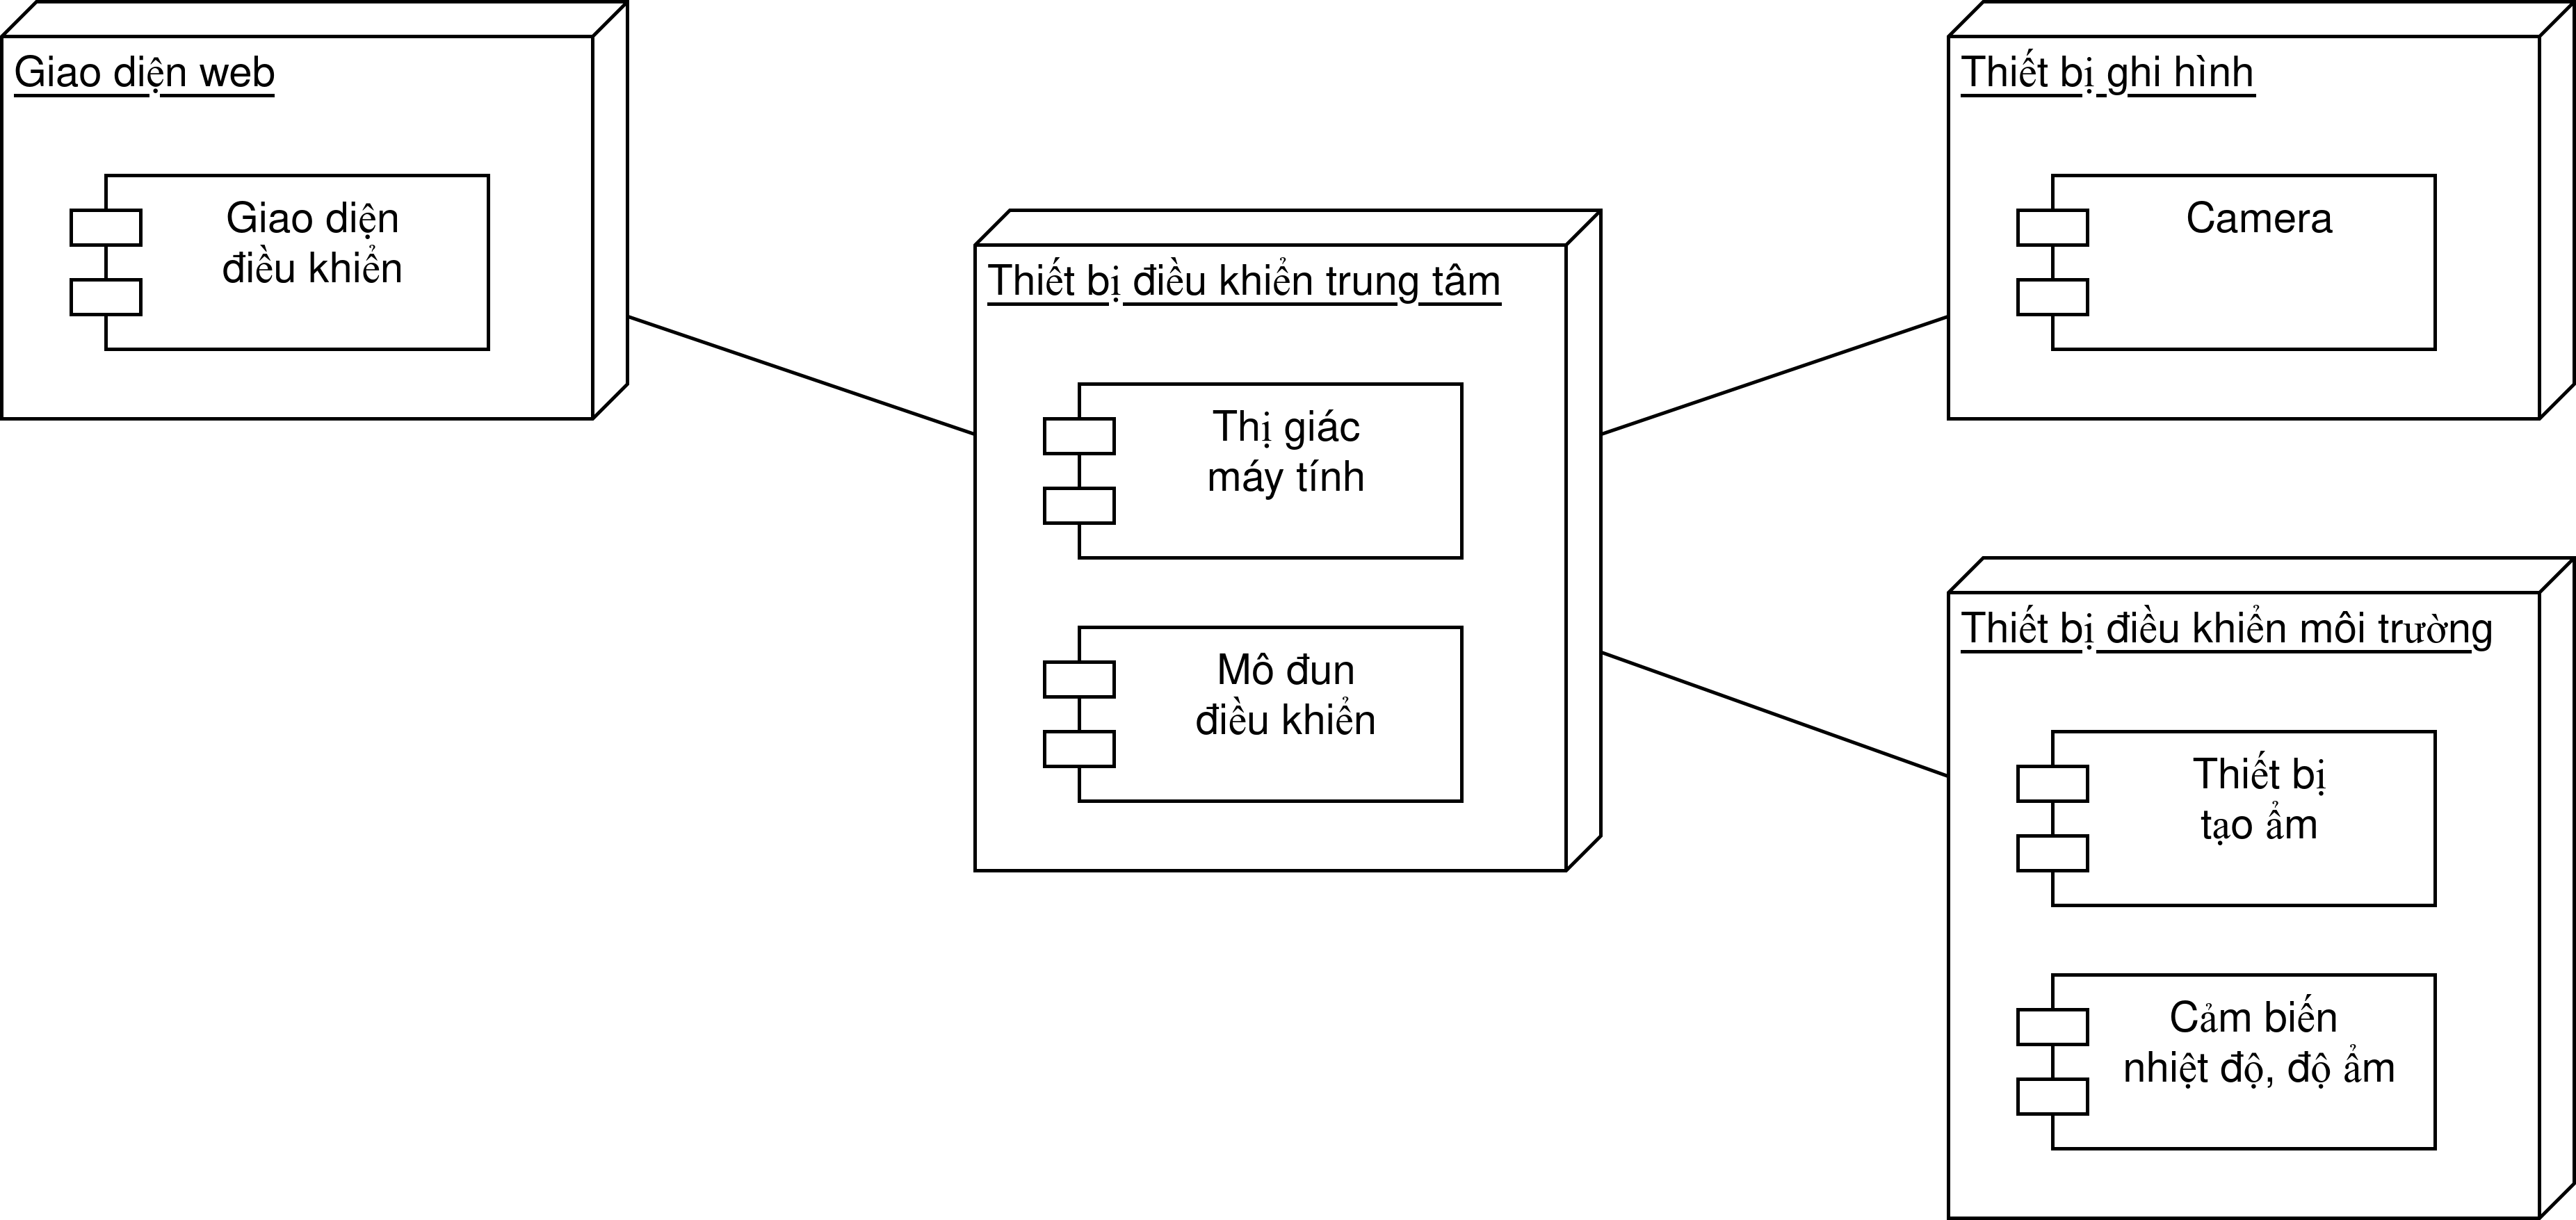
\includegraphics[width=0.75\linewidth]{images/deploy.png}
    \caption{Sơ đồ triển khai hệ thống}
    \label{fig:deploy}
\end{figure}

\subsection{Thiết kế phần mềm}

Phần mềm được chia thành các mô đun nhỏ thực hiện các chức năng khác nhau (Hình \ref{fig:software-component}).

\begin{itemize}
    \item Mô đun nhận hình ảnh thực hiện lấy hình ảnh từ Camera IP về thiết bị.
    \item Mô đun xử lý hình ảnh thực hiện phân tích hình ảnh bằng thị giác máy tính, giúp phát hiện và đưa ra vị trí nấm.
    \item Mô đun điều khiển tưới nước thực hiện bật tắt thiết bị tạo ẩm.
    \item Mô đun giao tiếp tạo diao diện kết nối giữa người dùng và mô đun điều khiển.
    \item Mô đun điều khiển thực hiện ghép nối các thành phần và gọi các mô đun tương ứng.
    \item Giao diện hiển thị hiển thị trạng thái hệ thống cho người quản lý.
\end{itemize}

\begin{figure}
    \centering
    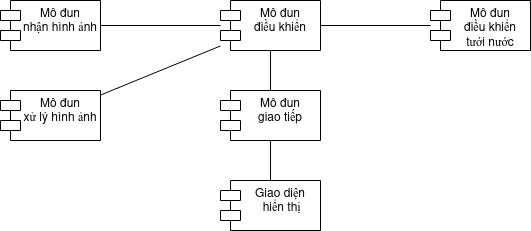
\includegraphics[width=0.75\linewidth]{images/software-component.png}
    \caption{Các thành phần phần mềm}
    \label{fig:software-component}
\end{figure}

\begin{figure}
    \centering
    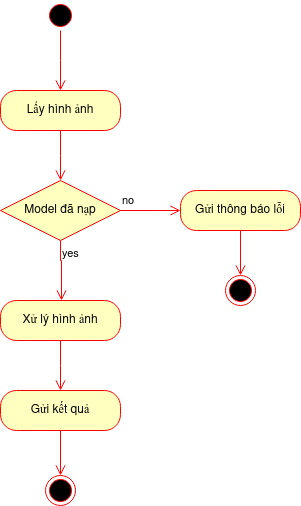
\includegraphics[width=0.55\linewidth]{images/vision-actvity.png}
    \caption{Biểu đồ hoạt động tác vụ phát hiện nấm}
    \label{fig:vision-activity}
\end{figure}


\begin{figure}[H]
    \centering
    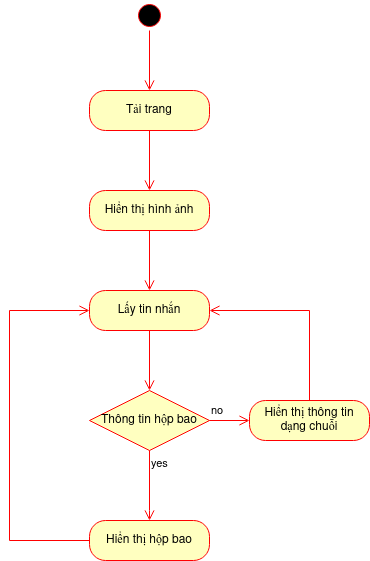
\includegraphics[width=0.55\linewidth]{images/ui-activity.png}
    \caption{Biểu đồ hoạt động giao diện người dùng}
    \label{fig:ui-activity}
\end{figure}

Việc chia nhỏ các tác vụ và thực hiện chúng song song có thể tối ưu hóa hiệu suất của ứng dụng. Khi các tác vụ không phụ thuộc vào nhau và có thể được thực hiện độc lập, ta có thể thực hiện chúng cùng một lúc trên nhiều luồng hoặc tiến trình, tận dụng được tài nguyên phần cứng và giảm thời gian thực thi.

Phần mềm được lập trình trên ngôn ngữ Rust, giúp việc lập trình song song trở nên đơn giản và an toàn hơn \cite{rust2022}. Ngoài ra, việc sử dụng ngôn ngữ lập trình biên dịch cùng các chế độ tối ưu hóa cũng giúp chương trình có hiệu suất cao hơn so với các ngôn ngữ thông dịch như Python.

\section{Xây dựng tập dữ liệu và huấn luyện mô hình}

\subsection{Thu thập dữ liệu}

Ngoài dữ liệu hình ảnh thu được trong thực tế trồng nấm, nguồn ảnh huấn luyện có thể thu thập từ nguồn mạng xã hội.

Roboflow là một nền tảng hỗ trợ tốt cho việc chuẩn bị dữ liệu huấn luyện. Dữ liệu huấn luyện có thể được tải lên Roboflow dưới dạng ảnh hoặc dạng video sau đó chuyển thành từng khung hình.


\subsection{Tiền xử lý và chuẩn bị dữ liệu huấn luyện}

Sau khi chuẩn bị dữ liệu huấn luyện, thực hiện gán nhãn cho từng vật thể (Hình \ref{fig:labeling-interface}).

\begin{figure}[H]]
    \centering
    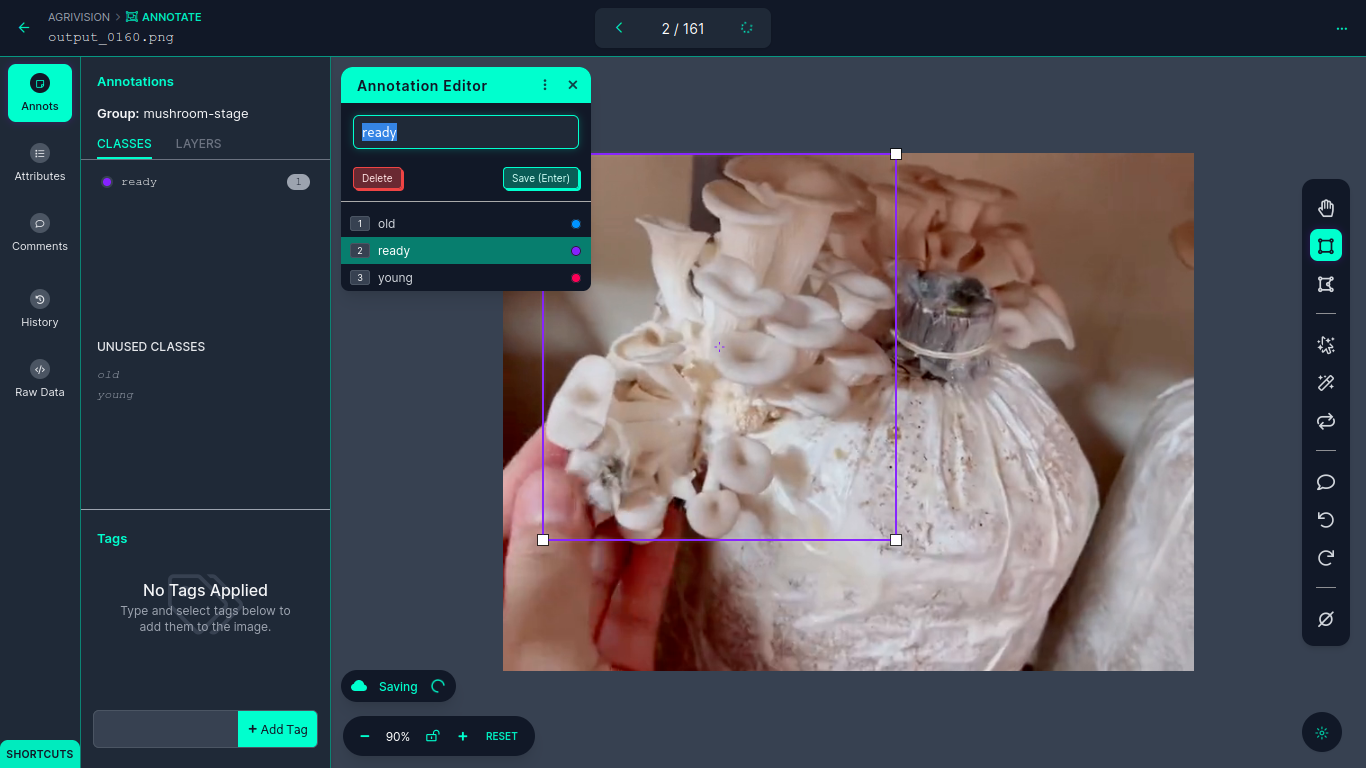
\includegraphics[width=0.85\linewidth]{images/image-labeling.png}
    \caption{Giao diện gán nhãn cho vật thể}
    \label{fig:labeling-interface}
\end{figure}

Nấm non có thân mọc thẳng về các phía, kích thước tai nấm không lớn hơn thân đáng kể (Hình \ref{fig:young}).

\begin{figure}[H]
    \centering
        \begin{subfigure}{.5\textwidth}
        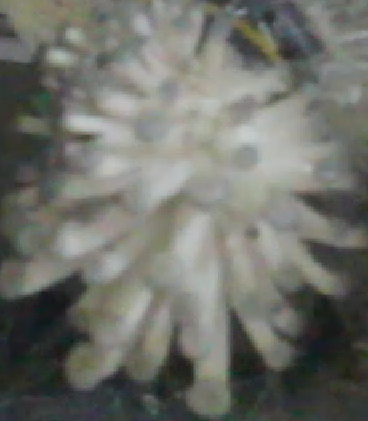
\includegraphics[width=0.8\linewidth]{images/young2.png}
    \end{subfigure}%
    \begin{subfigure}{.5\textwidth}
        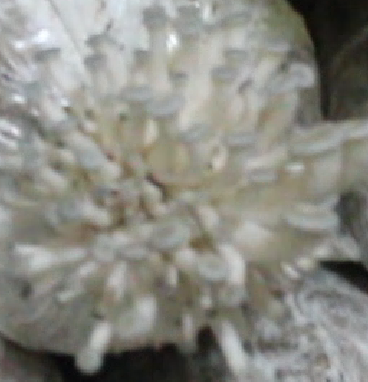
\includegraphics[width=0.8\linewidth]{images/young3.png}
    \end{subfigure}
    \caption{Hình ảnh nấm non}
    \label{fig:young}
\end{figure}

Nấm trưởng thành có tai nấm phát triển, thân nấm uốn cong lên phía trên (Hình \ref{fig:ready}).

\begin{figure}[H]
    \centering
        \begin{subfigure}{.5\textwidth}
        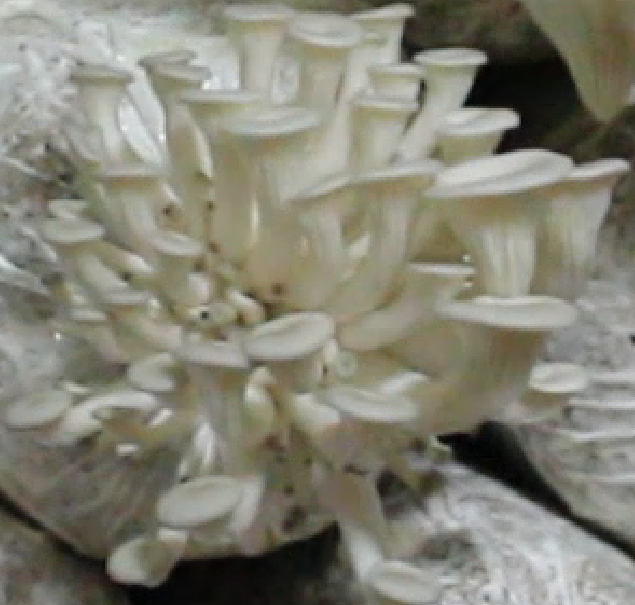
\includegraphics[width=0.8\linewidth]{images/ready1.png}
    \end{subfigure}%
    \begin{subfigure}{.5\textwidth}
        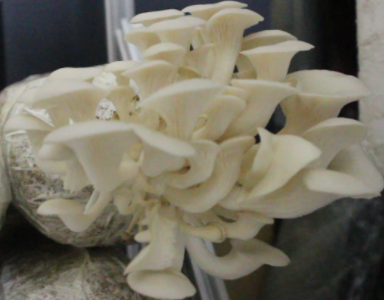
\includegraphics[width=0.8\linewidth]{images/ready3.png}
    \end{subfigure}
    \caption{Hình ảnh nấm trưởng thành, có thể thu hoạch}
    \label{fig:ready}
\end{figure}

Nấm già tai nấm phát triển to có thể bị xoăn lại và chuyển sang màu vàng., thân nấm nhỏ (Hình \ref{fig:old}).
\begin{figure}[H]
    \centering
    \begin{subfigure}{.5\textwidth}
        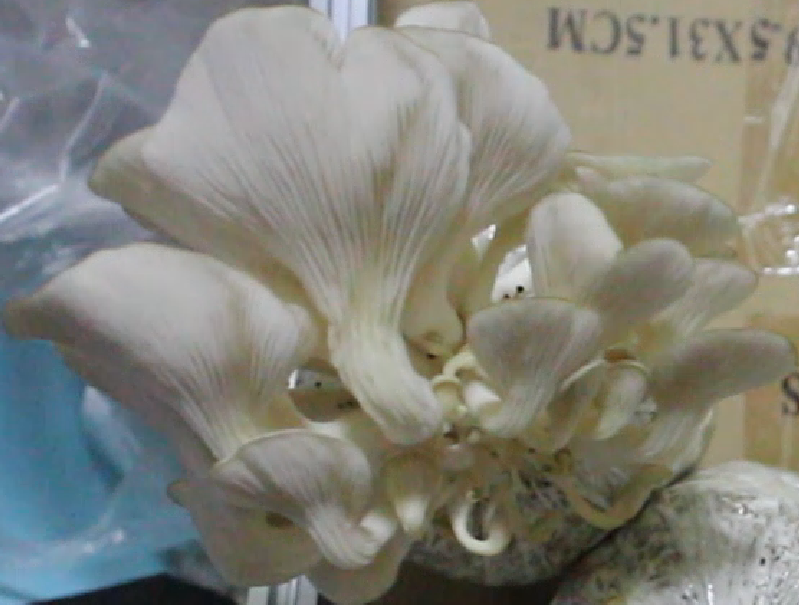
\includegraphics[width=0.85\linewidth]{images/old1.png}
    \end{subfigure}%
    \begin{subfigure}{.5\textwidth}
        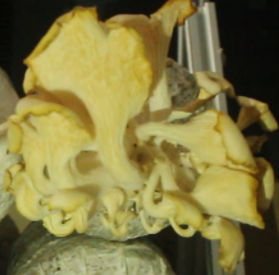
\includegraphics[width=0.85\linewidth]{images/old3.png}
    \end{subfigure}
    \caption{Hình ảnh nấm già}
    \label{fig:old}
\end{figure}

Dữ liệu huấn luyện sau khi chuẩn bị đầy đủ có thể được tải về và đưa vào huấn luyện (Hình \ref{fig:export-dataset}).
\begin{figure}[H]
    \centering
    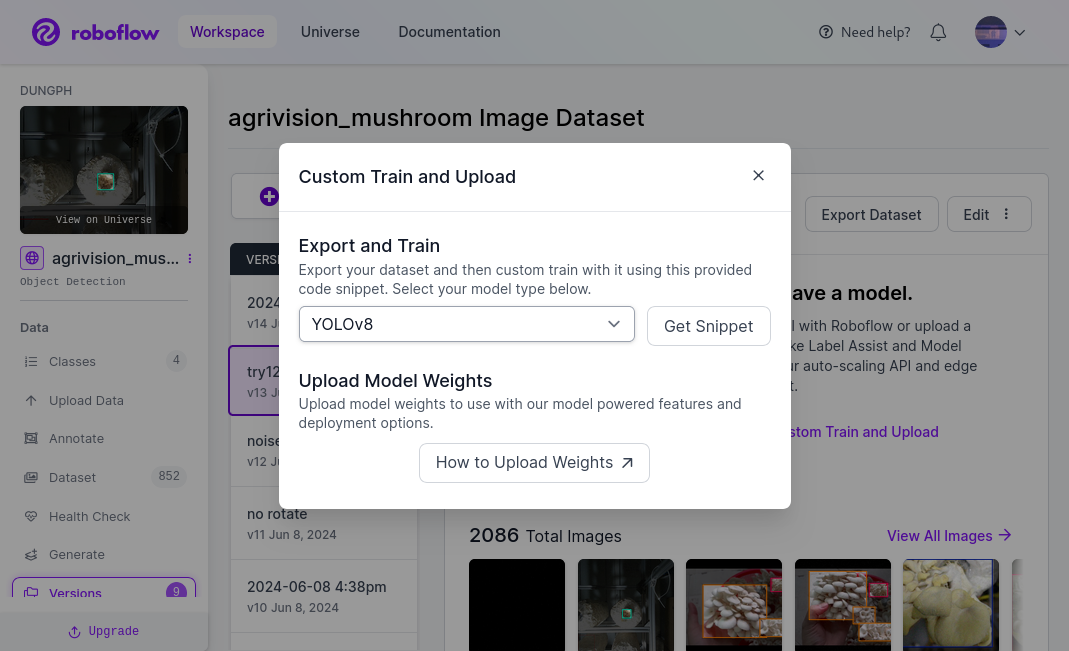
\includegraphics[width=0.85\linewidth]{images/export-dataset.png}
    \caption{Xuất tập dữ liệu huấn luyện}
    \label{fig:export-dataset}
\end{figure}

Tổng số nhãn gán cho ảnh bao gồm khoảng 2500 nấm non, 2500 nấm trưởng thành và 750 nấm già (Hình \ref{fig:instances-graph}).
\begin{figure}
    \centering
    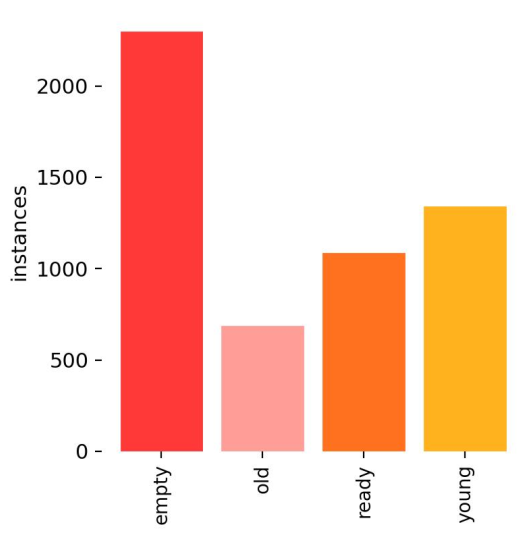
\includegraphics[width=0.55\linewidth]{images/instances-graph.png}
    \caption{Thống kê số lượng nhãn}
    \label{fig:instances-graph}
\end{figure}


Tổng số ảnh chuẩn bị cho huấn luyện là 753 ảnh. Sau quá trình tăng cường dữ liệu nghiêng ảnh và thêm nhiễu, số ảnh phục vụ huấn luyện là 1809 bao gồm 1586 ảnh huấn luyện, 152 ảnh giám sát và 71 ảnh kiểm thử.


\subsection{Huấn luyện và đánh giá hiệu suất mô hình}

Mô hình thị giác máy tính có thể được thực hiện nhờ google colab (Hình \ref{fig:colab-ui}.

\begin{figure}[h]
    \centering
    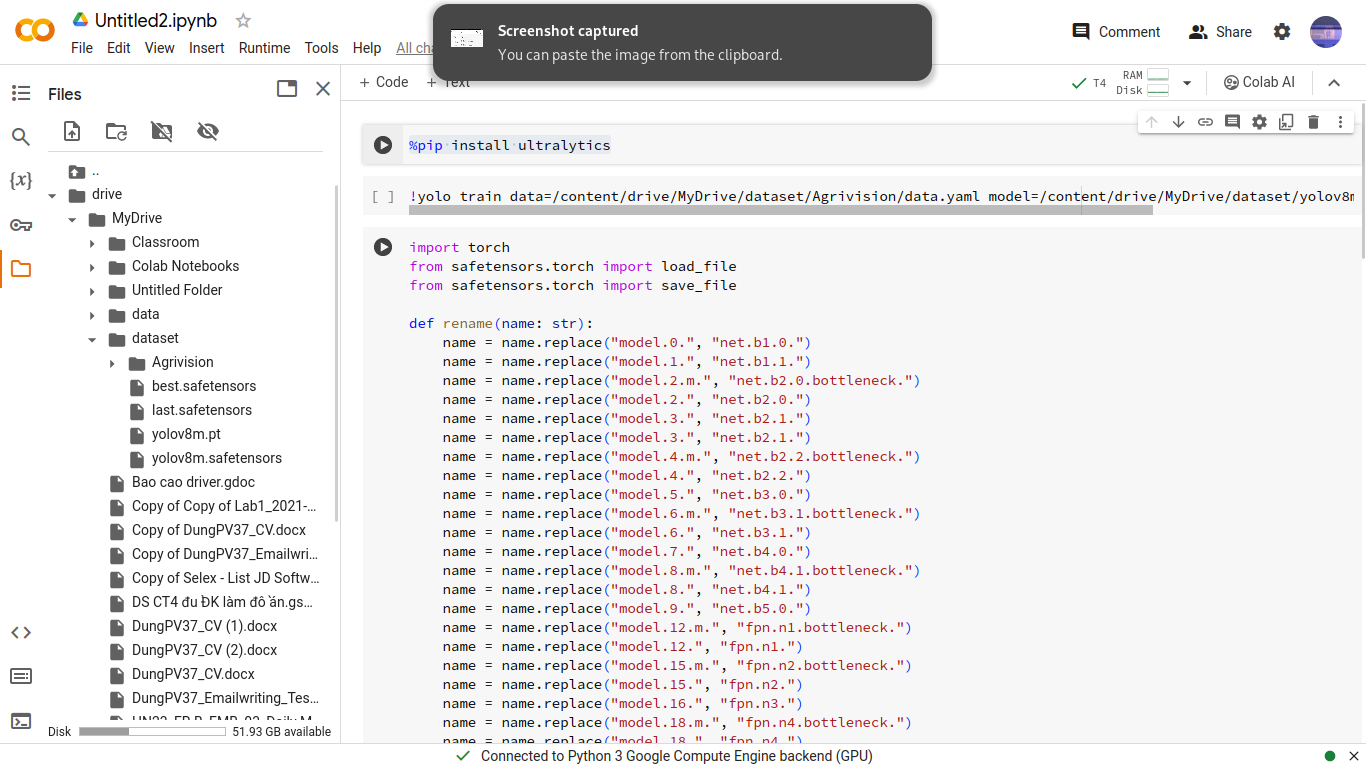
\includegraphics[width=0.85\linewidth]{images/colab-inteface.png}
    \caption{Giao diện Google Colab và mã nguồn}
    \label{fig:colab-ui}
\end{figure}

Nhập các thư viện YOLOv8:
\begin{lstlisting}
    %pip install ultralytics
\end{lstlisting}

Bắt đầu huấn luyện với các tham số:

\begin{itemize}
    \item train: Tác vụ huấn luyện
    \item data: Nơi lưu trữ tập dữ liệu tải từ Roboflow
    \item model: Kích thước model sử dụng, X là lớn nhất, s là nhỏ, n là nhỏ nhất. Do dữ liệu huấn luyện có số lượng nhỏ nên sử dụng n để tránh overfiting.
    \item epochs: Số vòng huấn luyện. Thử từ 50 epoch do số lượng dữ liệu huấn luyện nhỏ.
\end{itemize}
\begin{lstlisting}
!yolo train data=data.yaml model=yolov8n.pt epochs=50 lr0=0.01
\end{lstlisting}

Chuyển mô hình huấn luyện được về dạng safetensors và chỉnh sửa mô hình để chạy trên Candle:
\begin{lstlisting}[language=python]
import torch
from safetensors.torch import load_file
from safetensors.torch import save_file

def rename(name: str):
    name = name.replace("model.0.", "net.b1.0.")
    name = name.replace("model.1.", "net.b1.1.")
    name = name.replace("model.2.m.", "net.b2.0.bottleneck.")
    name = name.replace("model.2.", "net.b2.0.")
    name = name.replace("model.3.", "net.b2.1.")
    name = name.replace("model.3.", "net.b2.1.")
    name = name.replace("model.4.m.", "net.b2.2.bottleneck.")
    name = name.replace("model.4.", "net.b2.2.")
    name = name.replace("model.5.", "net.b3.0.")
    name = name.replace("model.6.m.", "net.b3.1.bottleneck.")
    name = name.replace("model.6.", "net.b3.1.")
    name = name.replace("model.7.", "net.b4.0.")
    name = name.replace("model.8.m.", "net.b4.1.bottleneck.")
    name = name.replace("model.8.", "net.b4.1.")
    name = name.replace("model.9.", "net.b5.0.")
    name = name.replace("model.12.m.", "fpn.n1.bottleneck.")
    name = name.replace("model.12.", "fpn.n1.")
    name = name.replace("model.15.m.", "fpn.n2.bottleneck.")
    name = name.replace("model.15.", "fpn.n2.")
    name = name.replace("model.16.", "fpn.n3.")
    name = name.replace("model.18.m.", "fpn.n4.bottleneck.")
    name = name.replace("model.18.", "fpn.n4.")
    name = name.replace("model.19.", "fpn.n5.")
    name = name.replace("model.21.m.", "fpn.n6.bottleneck.")
    name = name.replace("model.21.", "fpn.n6.")
    name = name.replace("model.22.", "head.")
    return name

data = torch.load("runs/detect/train5/weights/last.pt")
tensors = data['model'].state_dict().items()
tensors = dict(tensors)
tensors = {rename(k): t for k, t in tensors.items()}
print(data["model"])
save_file(tensors, "/runs/detect/train5/weights/last.safetensors")
for k, v in tensors.items():
    print(str(k), v.shape)
\end{lstlisting}

Từ hình \ref{fig:training-result-f1}, mô hình đưa ra kết quả chính xác nhất với hệ số tự tin từ 20\% đến 70\%, hệ số tự tin càng cao càng đưa ra kết quả chính xác trong hình \ref{fig:training-result-p} và tỉ lệ phát hiện đúng vật thể giảm rõ rệt khi hệ số tự tin lớn hơn 70\% (Hình \ref{fig:training-result-r}).

\begin{figure}
    \centering
    \begin{subfigure}{.5\textwidth}
        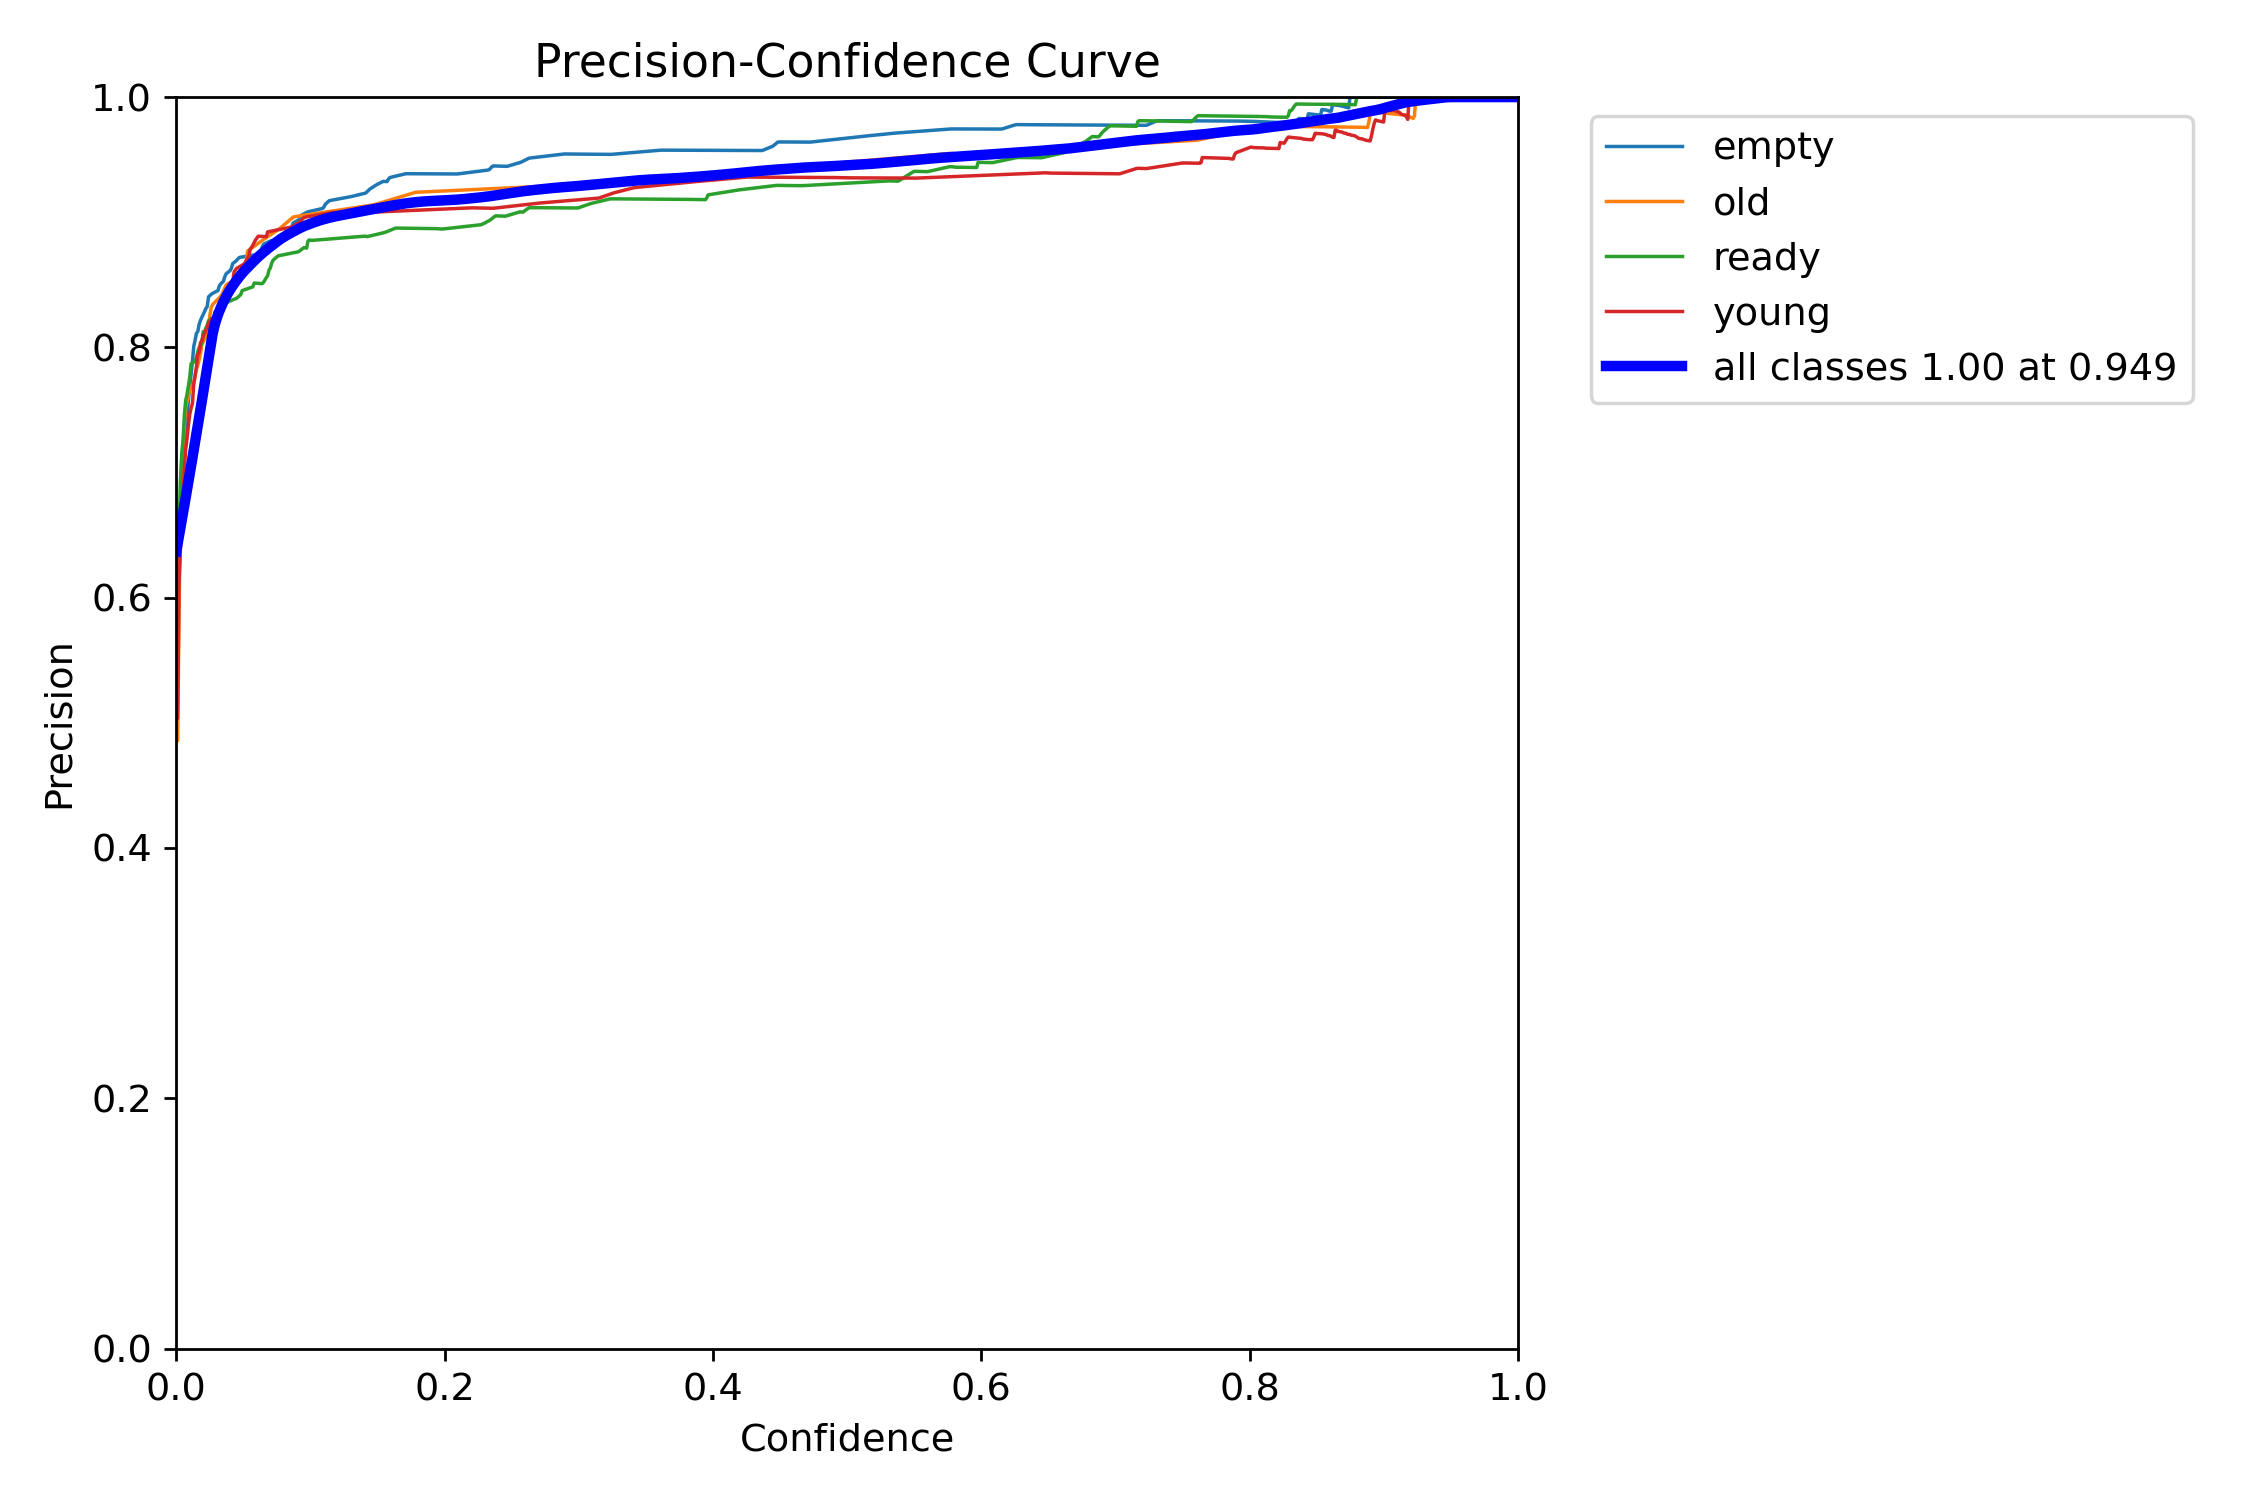
\includegraphics[width=0.95\linewidth]{images/P_curve.png}
    \caption{Đường cong Precision}
    \label{fig:training-result-p}

    \end{subfigure}%
    \begin{subfigure}{.5\textwidth}
        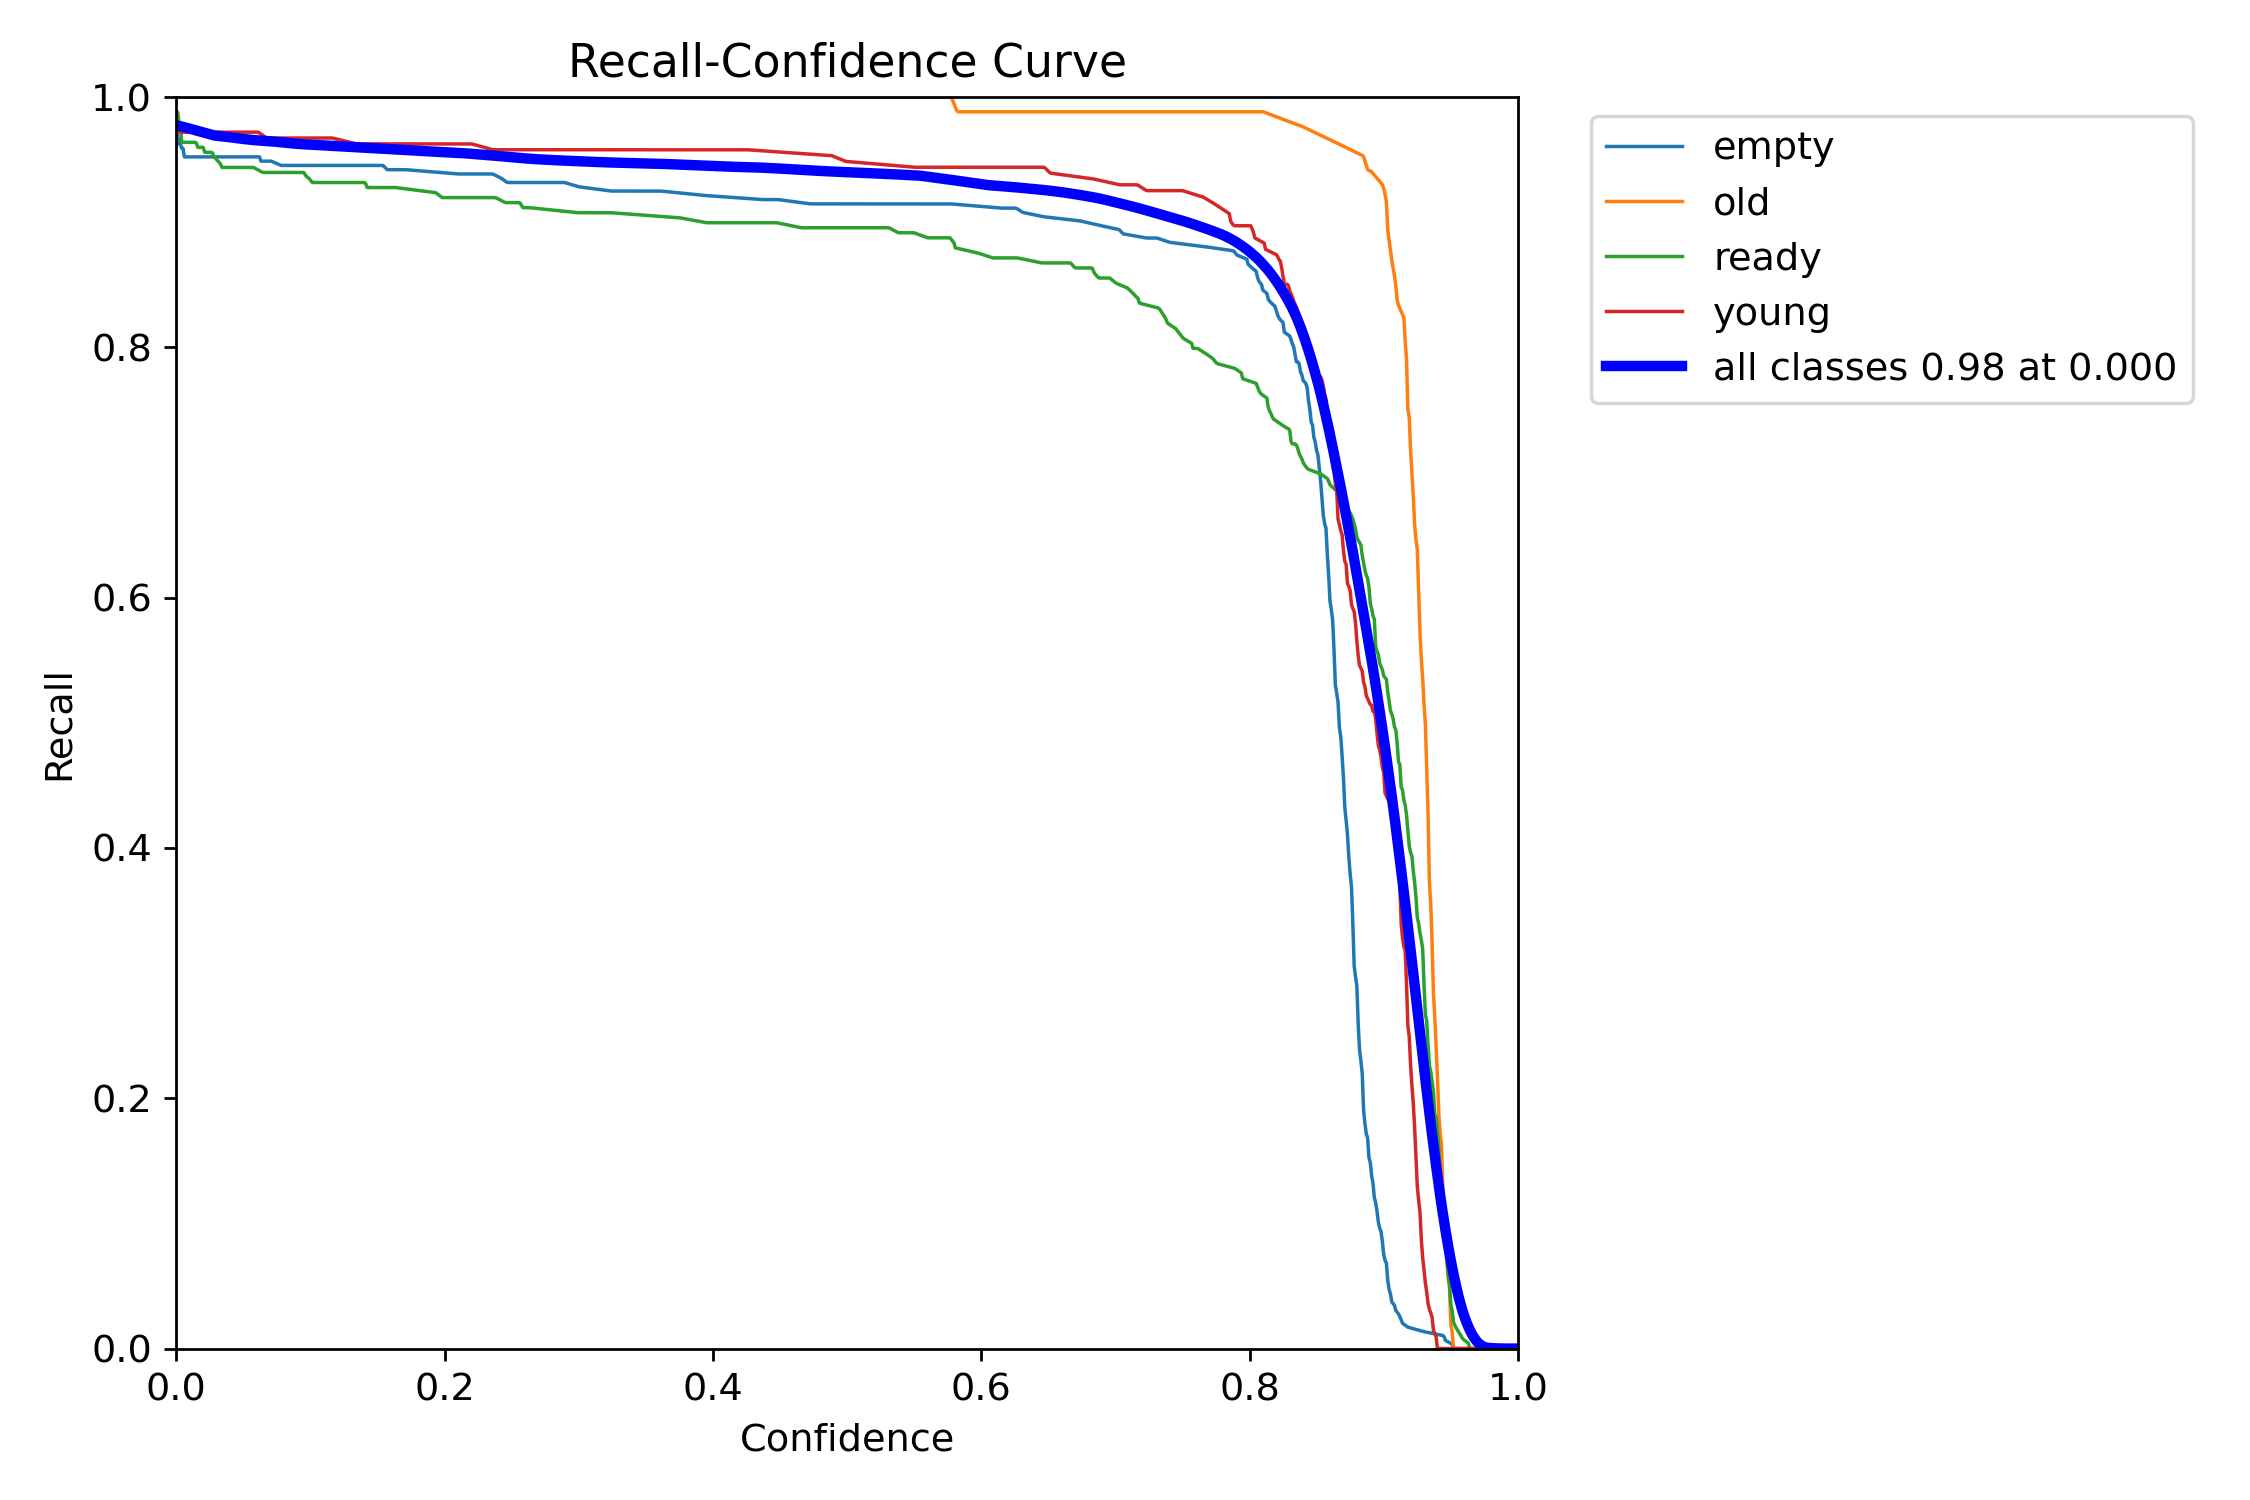
\includegraphics[width=0.95\linewidth]{images/R_curve.png}
    \caption{Đường cong Recall}
    \label{fig:training-result-r}
    \end{subfigure}
    \begin{subfigure}{.5\textwidth}
        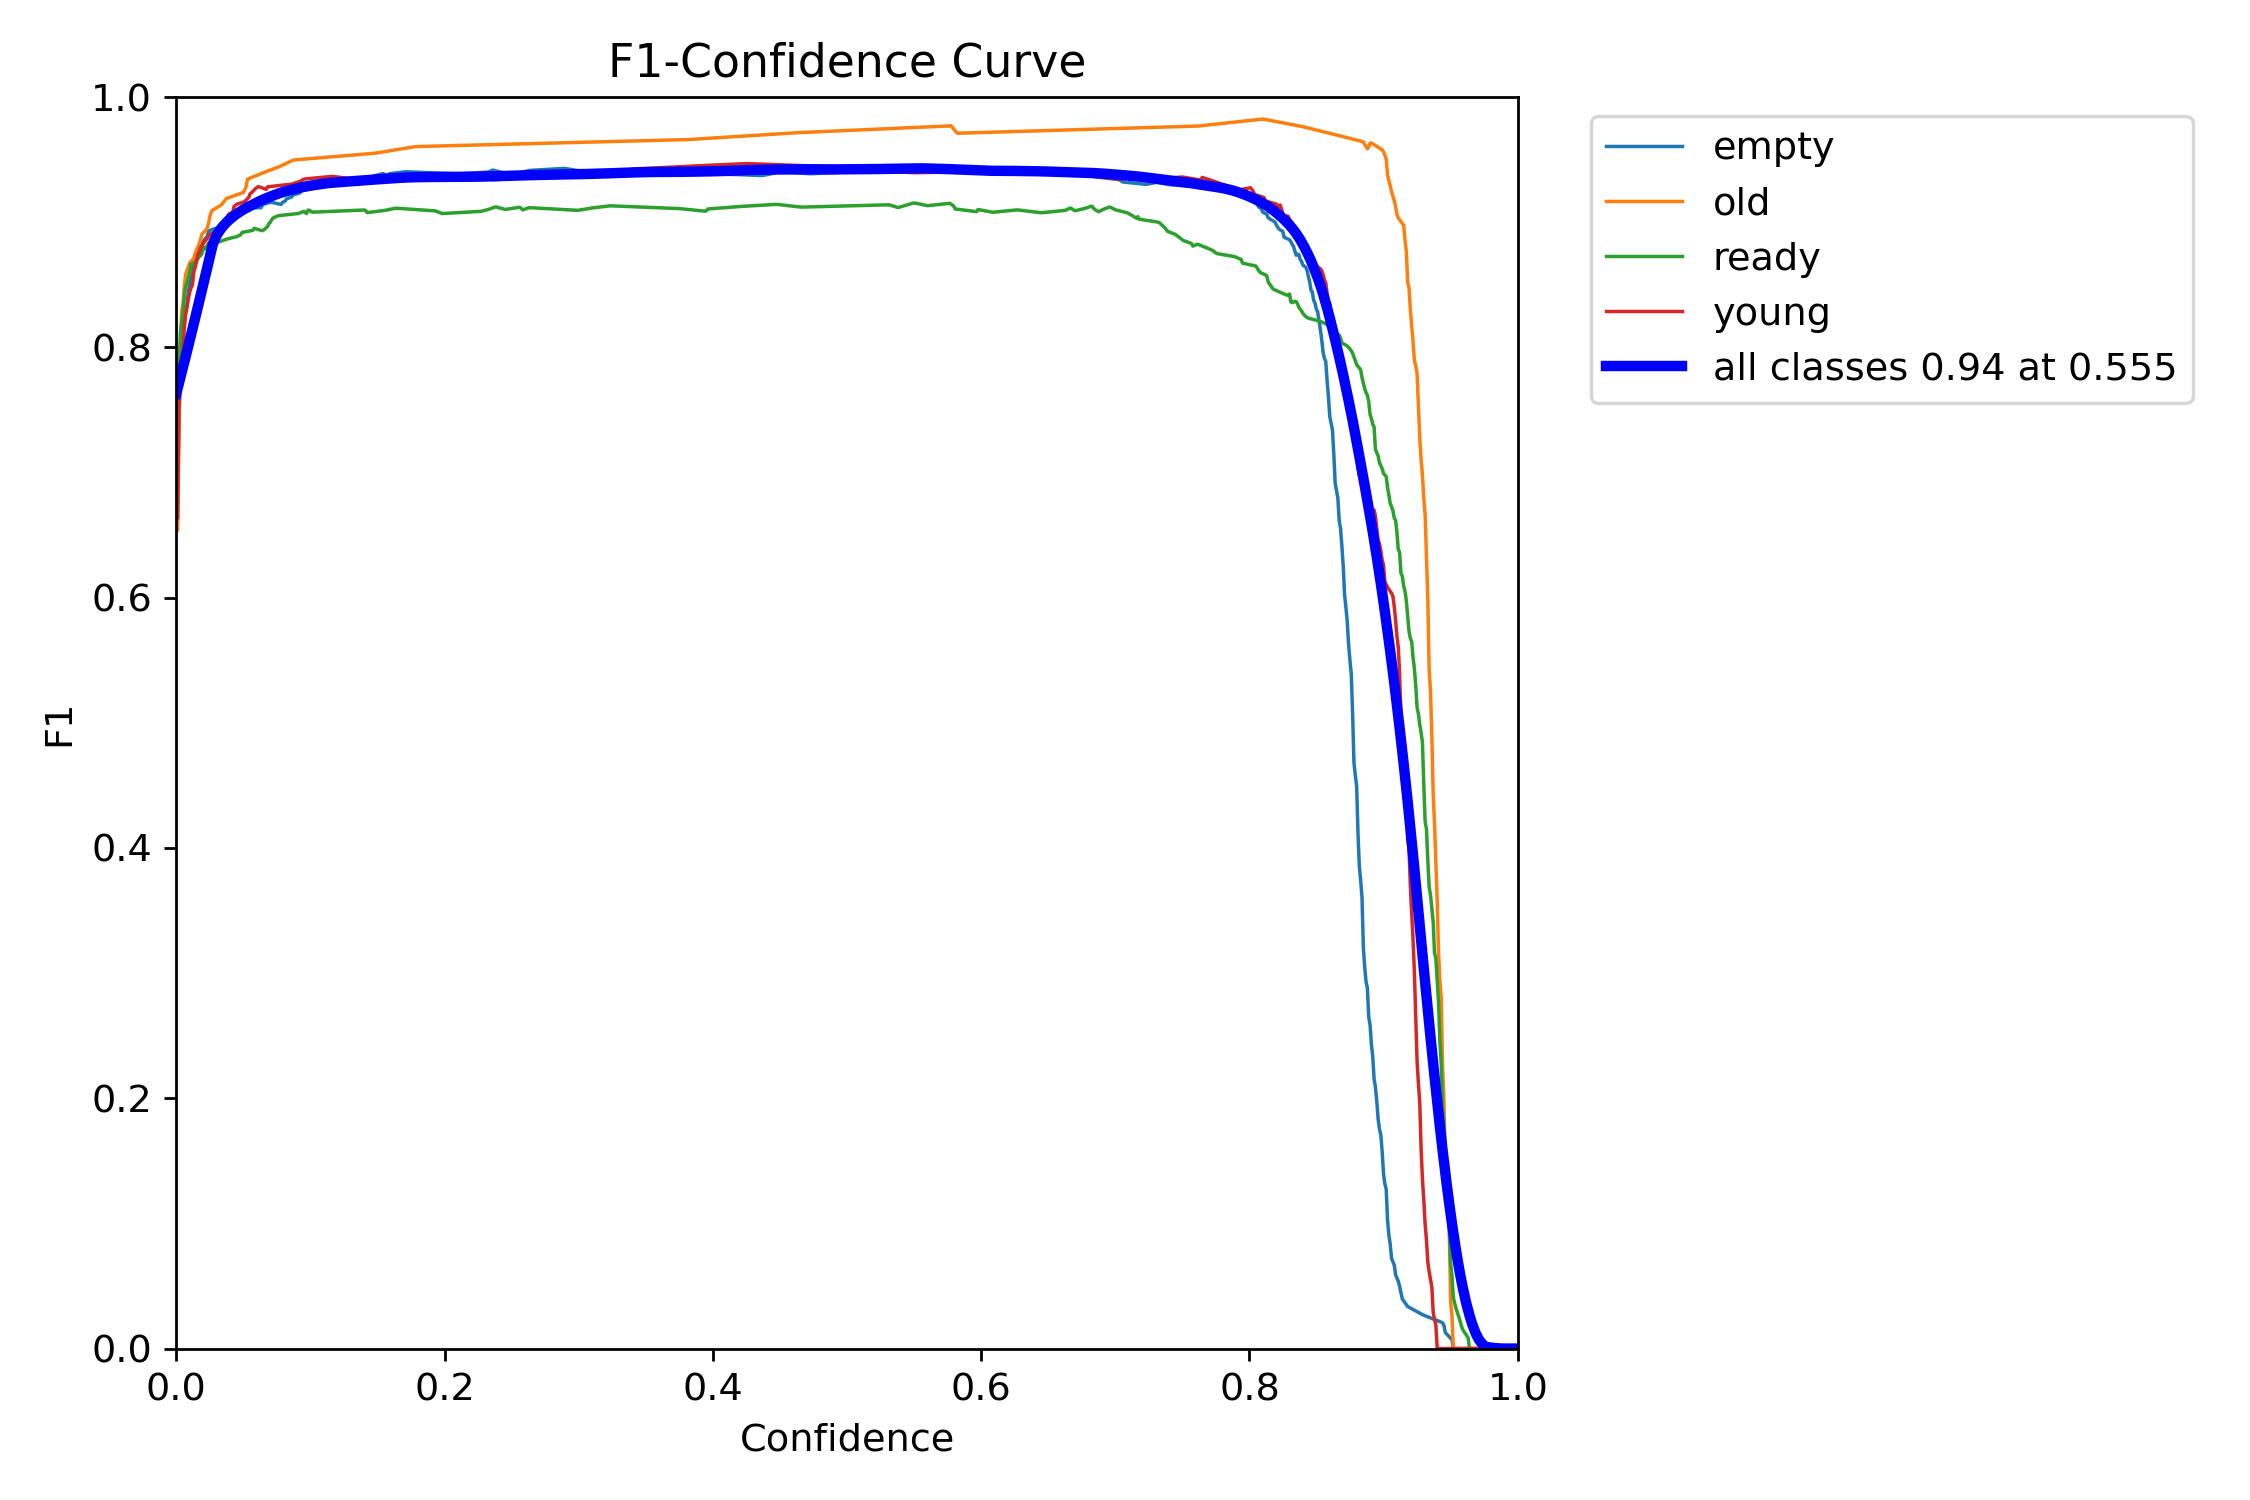
\includegraphics[width=0.95\linewidth]{images/F1_curve.png}
    \caption{Đường cong F1-score}
    \label{fig:training-result-f1}

    \end{subfigure}
    \caption{Kết quả huấn luyện}

    \label{fig:training-result}
\end{figure}

\begin{figure}[h]
    \centering
    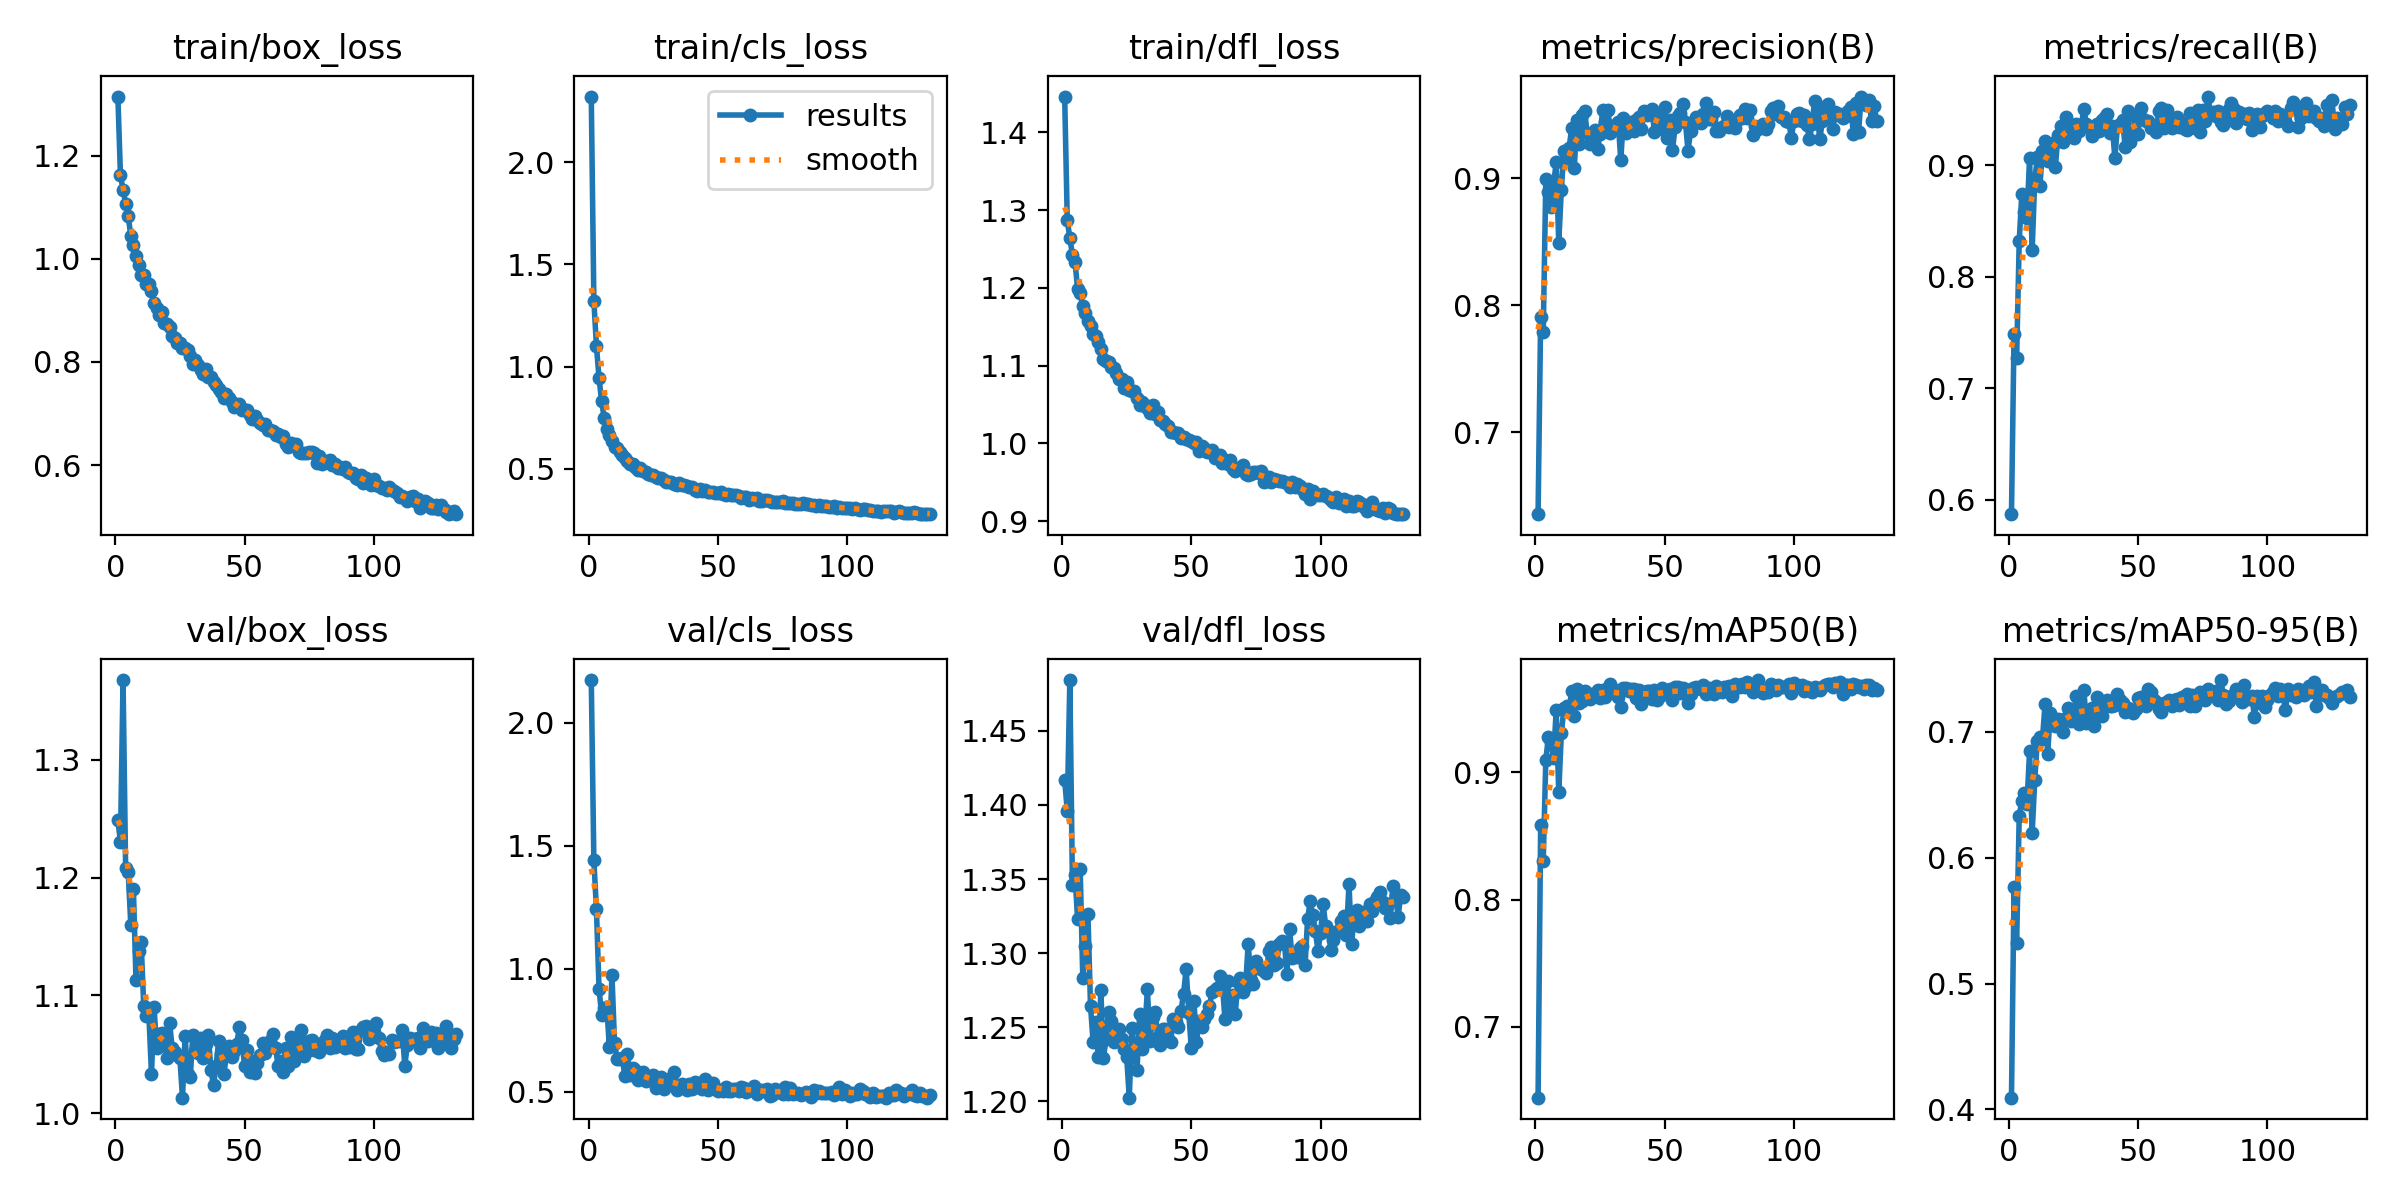
\includegraphics[width=0.85\linewidth]{images/results.png}
    \caption{Đồ thị mất mát}
    \label{fig:loss}
\end{figure}

Đồ thị \ref{fig:loss} cho thấy số lượng dữ liệu huấn luyện nhỏ nên gặp nhiều nhiều đỉnh trong đồ thị. Sau khoảng 40 vòng huấn luyện, đồ thị mất mát cho tác vụ xác định vị trí vẫn đang đi xuống với góc nghiêng nhỏ nên còn bị underfitting. Tuy nhiên, đồ thị mất mất cho tác vụ phân lớp gần như nằm ngang nên không bị overfitting hay underfitting. 

Ma trận thu (Hình \ref{fig:confusion-matrix}) cho thấy mô hình đoán nhận khá chính xác, tuy nhiên nhiều trường hợp không đoán nhận được nấm non do nhiều hình ảnh nấm quá non bị thiếu độ chi tiết, cần chỉnh sửa thêm.


\begin{figure}[H]
    \centering
    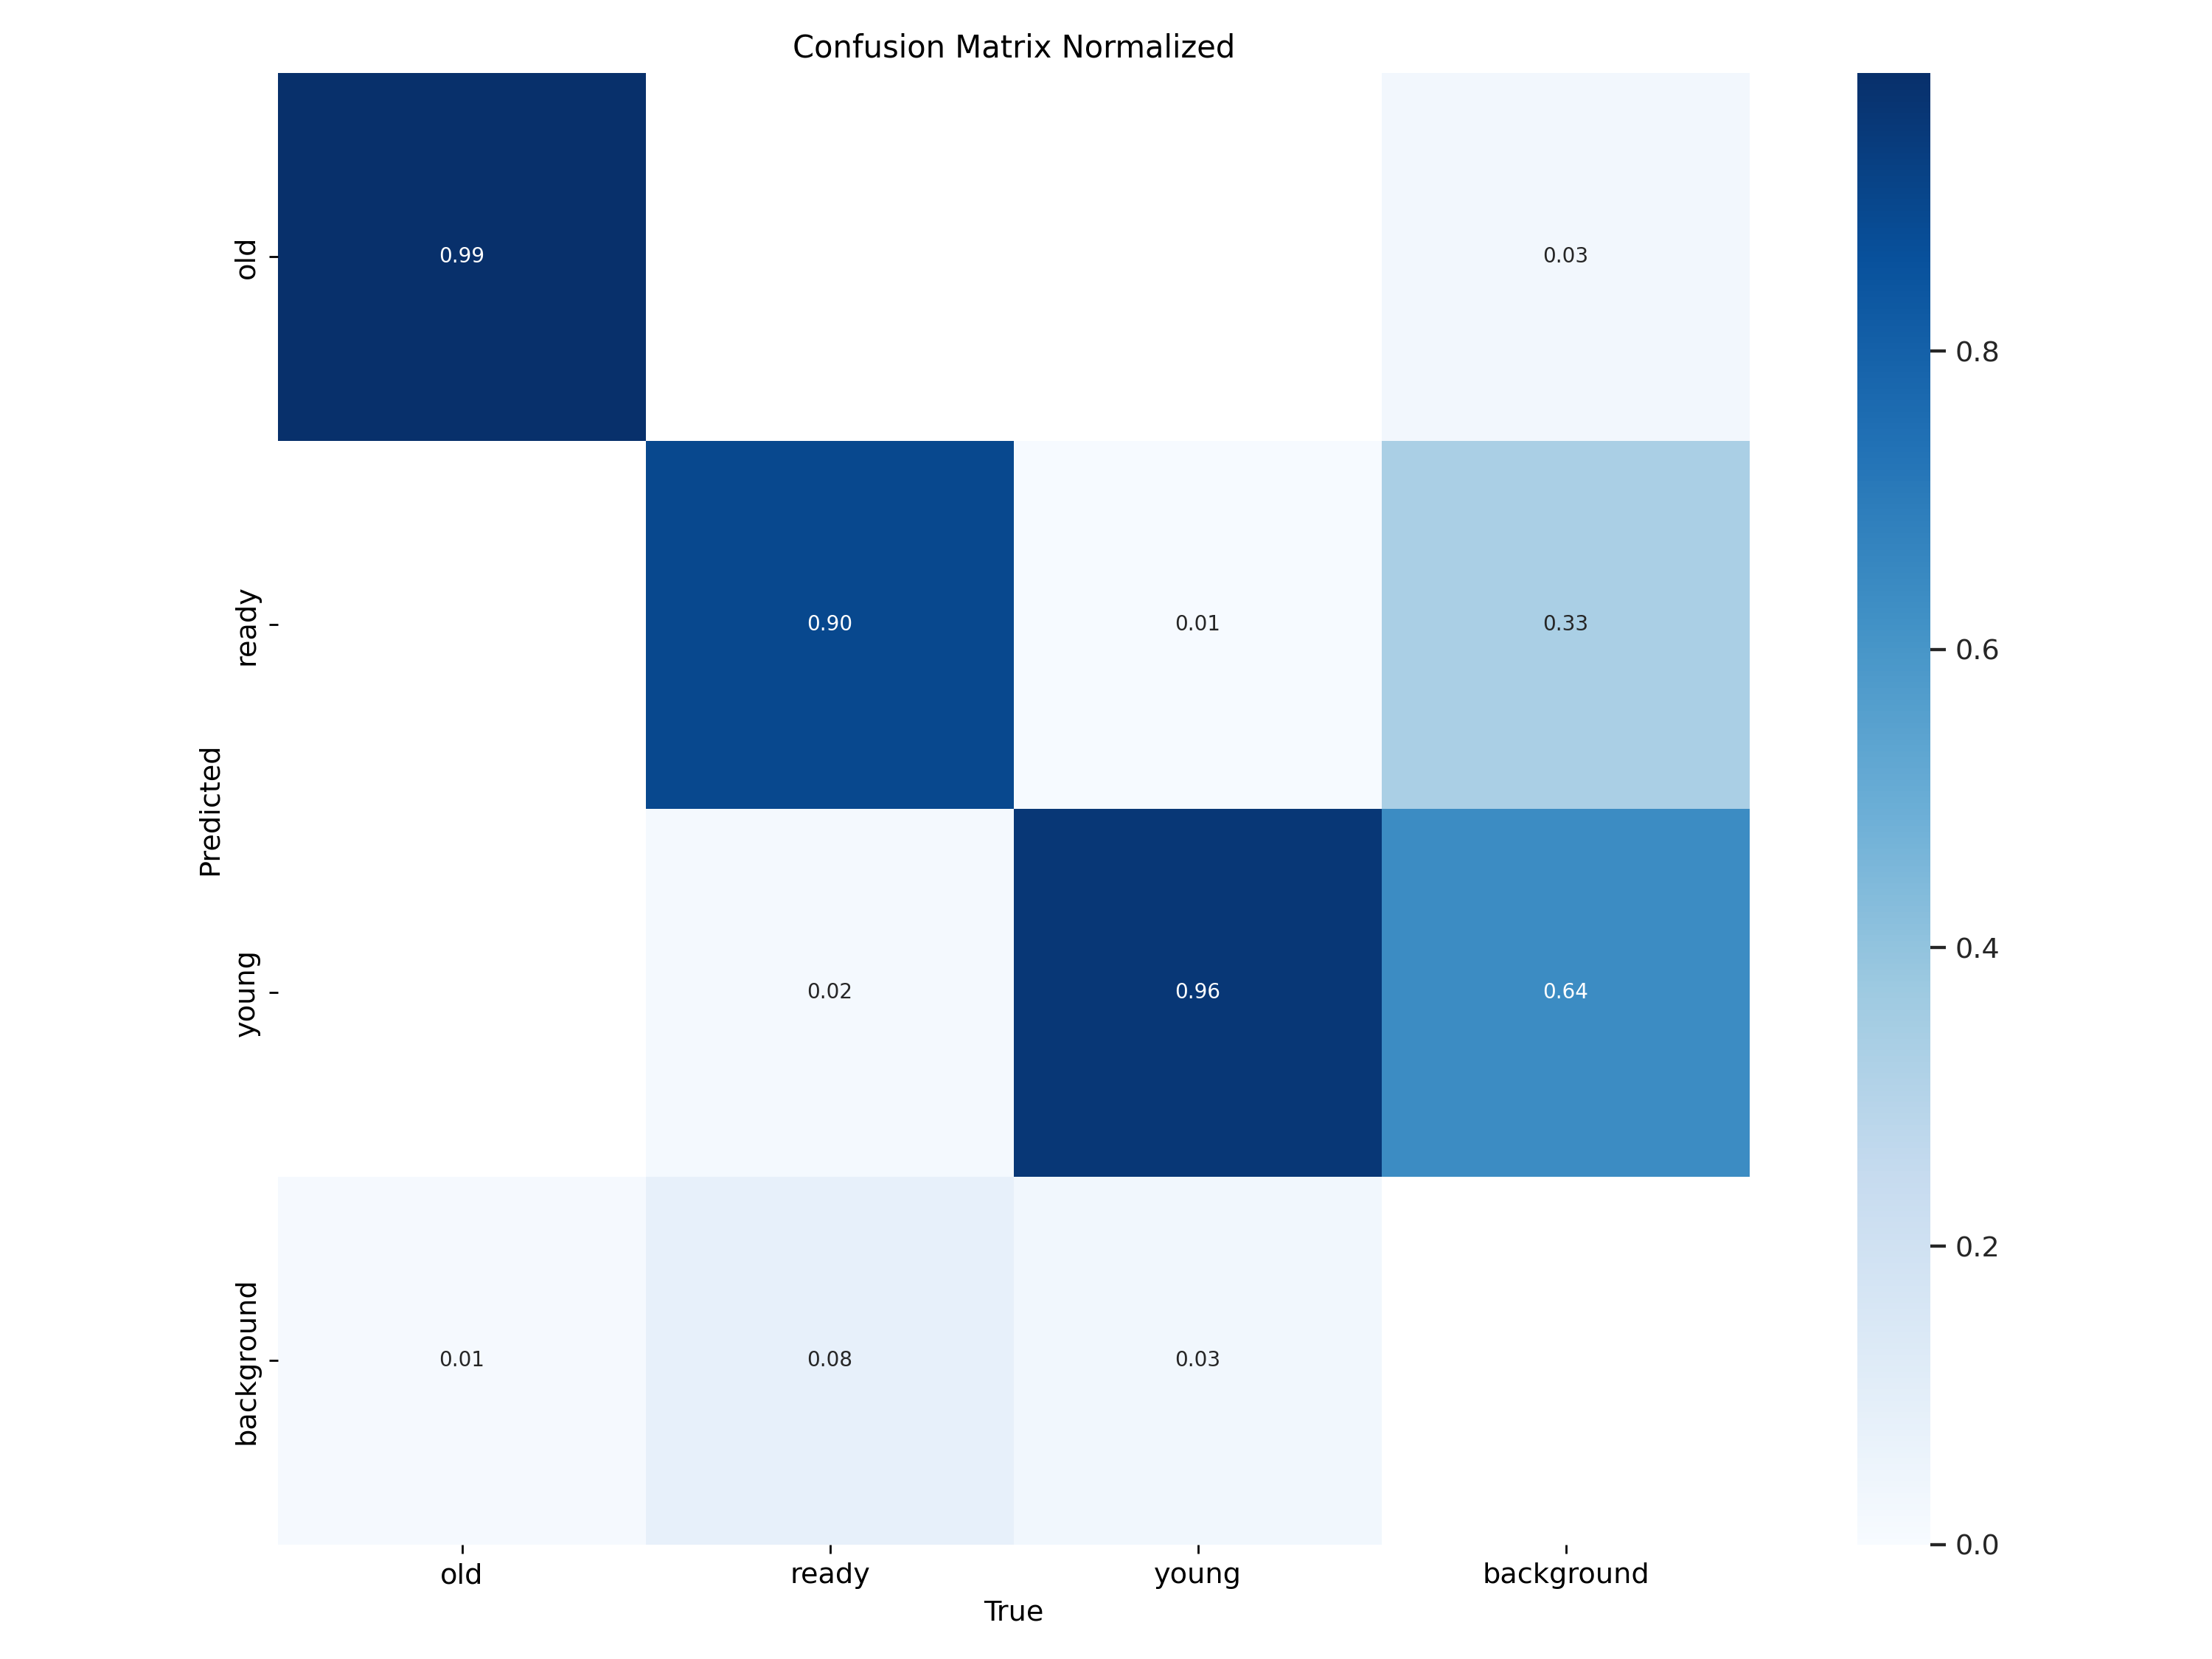
\includegraphics[width=0.85\linewidth]{images/confusion_matrix_normalized.png}
    \caption{Ma trận thu}
    \label{fig:confusion-matrix}
\end{figure}

\section{Tích hợp và tinh chỉnh hệ thống}
Sau khi huấn luyện, mô hình có thể được sử dụng trong hệ thống. 



\begin{table}[H]
\centering
\caption{Thông số chạy chương trình}
\label{tab:run-command}
\begin{tabular}{|l|l|l|}
\hline
\textbf{Thuộc tính} & \textbf{Giá trị mặc định} & \textbf{Mô tả}                     \\ \hline
--port              & {[}default: 8080{]}       & Cổng cho api                       \\ \hline
--model-path        &                           & Đường dẫn tới mô hình              \\ \hline
--model-size        & {[}default: m{]}          & Kích thước mô hình \\ \hline
--num-classes       & {[}default: 1{]}          & Số lớp nhận diện bởi mô            \\ \hline
--store-path        & {[}default: ./images{]}   & Đường dẫn lưu ảnh                  \\ \hline
--camera-device     &                           & Thiết bị camera                    \\ \hline
--snapshot-url      &                           & Đường dẫn lấy hình ảnh camera      \\ \hline
--stream-url        & {[}default: /video{]}     & Đường dẫn video camera             \\ \hline
--pump-pin          &                           & Chân gpio kết nối bơm              \\ \hline
--pump-on           & {[}default: 1{]}          & Thời gian bơm bật                  \\ \hline
--pump-off          & {[}default: 1{]}          & Thời gian bơm tắt                  \\ \hline
\end{tabular}
\end{table}

Giao diện người dùng hiển thị trạng thái hệ thống, hiển thị hình ảnh theo dõi và hộp bao tương ứng với kết quả tương đối chính xác với cả hộp bao và trạng thái sinh trưởng (Hình \ref{fig:user-interface}).
\begin{figure}[H]
    \centering
    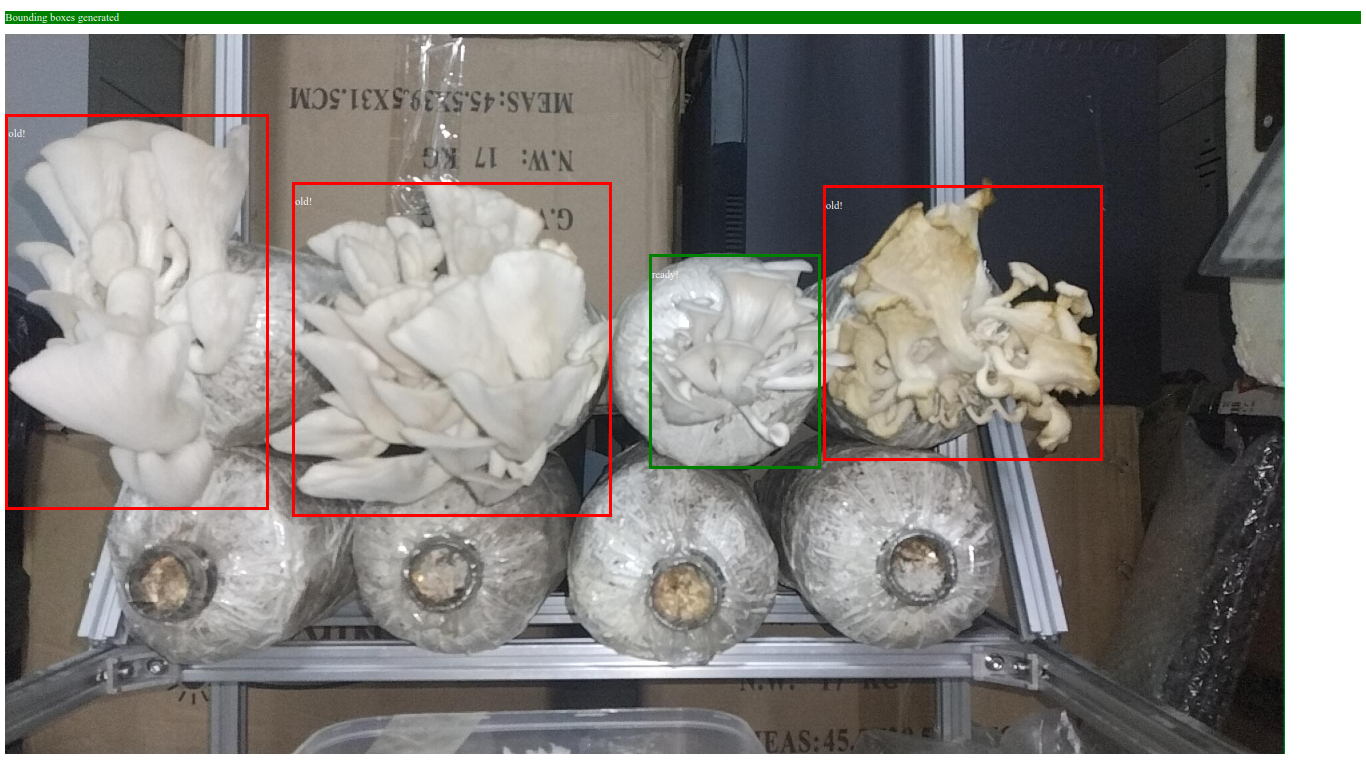
\includegraphics[width=0.75\linewidth]{images/user-interface.png}
    \caption{Giao diện nhận diện ảnh nấm}
    \label{fig:user-interface}
\end{figure}


\section{Tổng kết chương}

Trong chương 3, phần "Xây dựng hệ thống theo dõi và chăm sóc nấm" bao gồm sơ đồ triển khai hệ thống, bao gồm liên kết giữa các thành phần với nhau. 

Tiếp theo, phần "Xây dựng tập dữ liệu và huấn luyện mô hình" là quá trình xây dựng tập dữ liệu huấn luyện bao gồm:
\begin{itemize}
    \item Thu thập dữ liệu từ các nguồn khác nhau để đảm bảo độ đa dạng và đủ lớn cho quá trình huấn luyện.
    \item Tiền xử lý và chuẩn bị dữ liệu huấn luyện để đảm bảo chất lượng và độ tin cậy của dữ liệu.
    \item Huấn luyện mô hình và đánh giá hiệu suất của nó để đảm bảo rằng mô hình có khả năng phân loại các loại nấm một cách chính xác.
\end{itemize}

Cuối cùng, mô hình thị giác máy tính được tích hợp và chạy thử trong hệ thống với thành công bước đầu khi nhận diện trạng thái sinh trưởng của nấm thành công.